\chapter{系统设计与实现}

    系统的实现包括\textbf{核心工具Lapis}和辅助使用工具两大部分. 其中, Lapis工具提供从脚本解析到测试生成与执行的整套方法的原型实现. 辅助使用工具则有在线API脚本的上传、编辑和可视化web工具. 它们完全独立.

    % extended version
    % 原型系统包括核心工具Lapis和用户接口两大组件. 其中, 核心工具提供从脚本解析到测试生成与执行的整套方法的原型实现. 用户接口则包括核心工具的编程API接口, 和在线API脚本的上传、编辑和可视化的web应用, 以及桌面端测试管理系统. 以上各部分完全独立.

	\section{Lapis}
	
	    \begin{figure}[!htb]
	        \centering
	        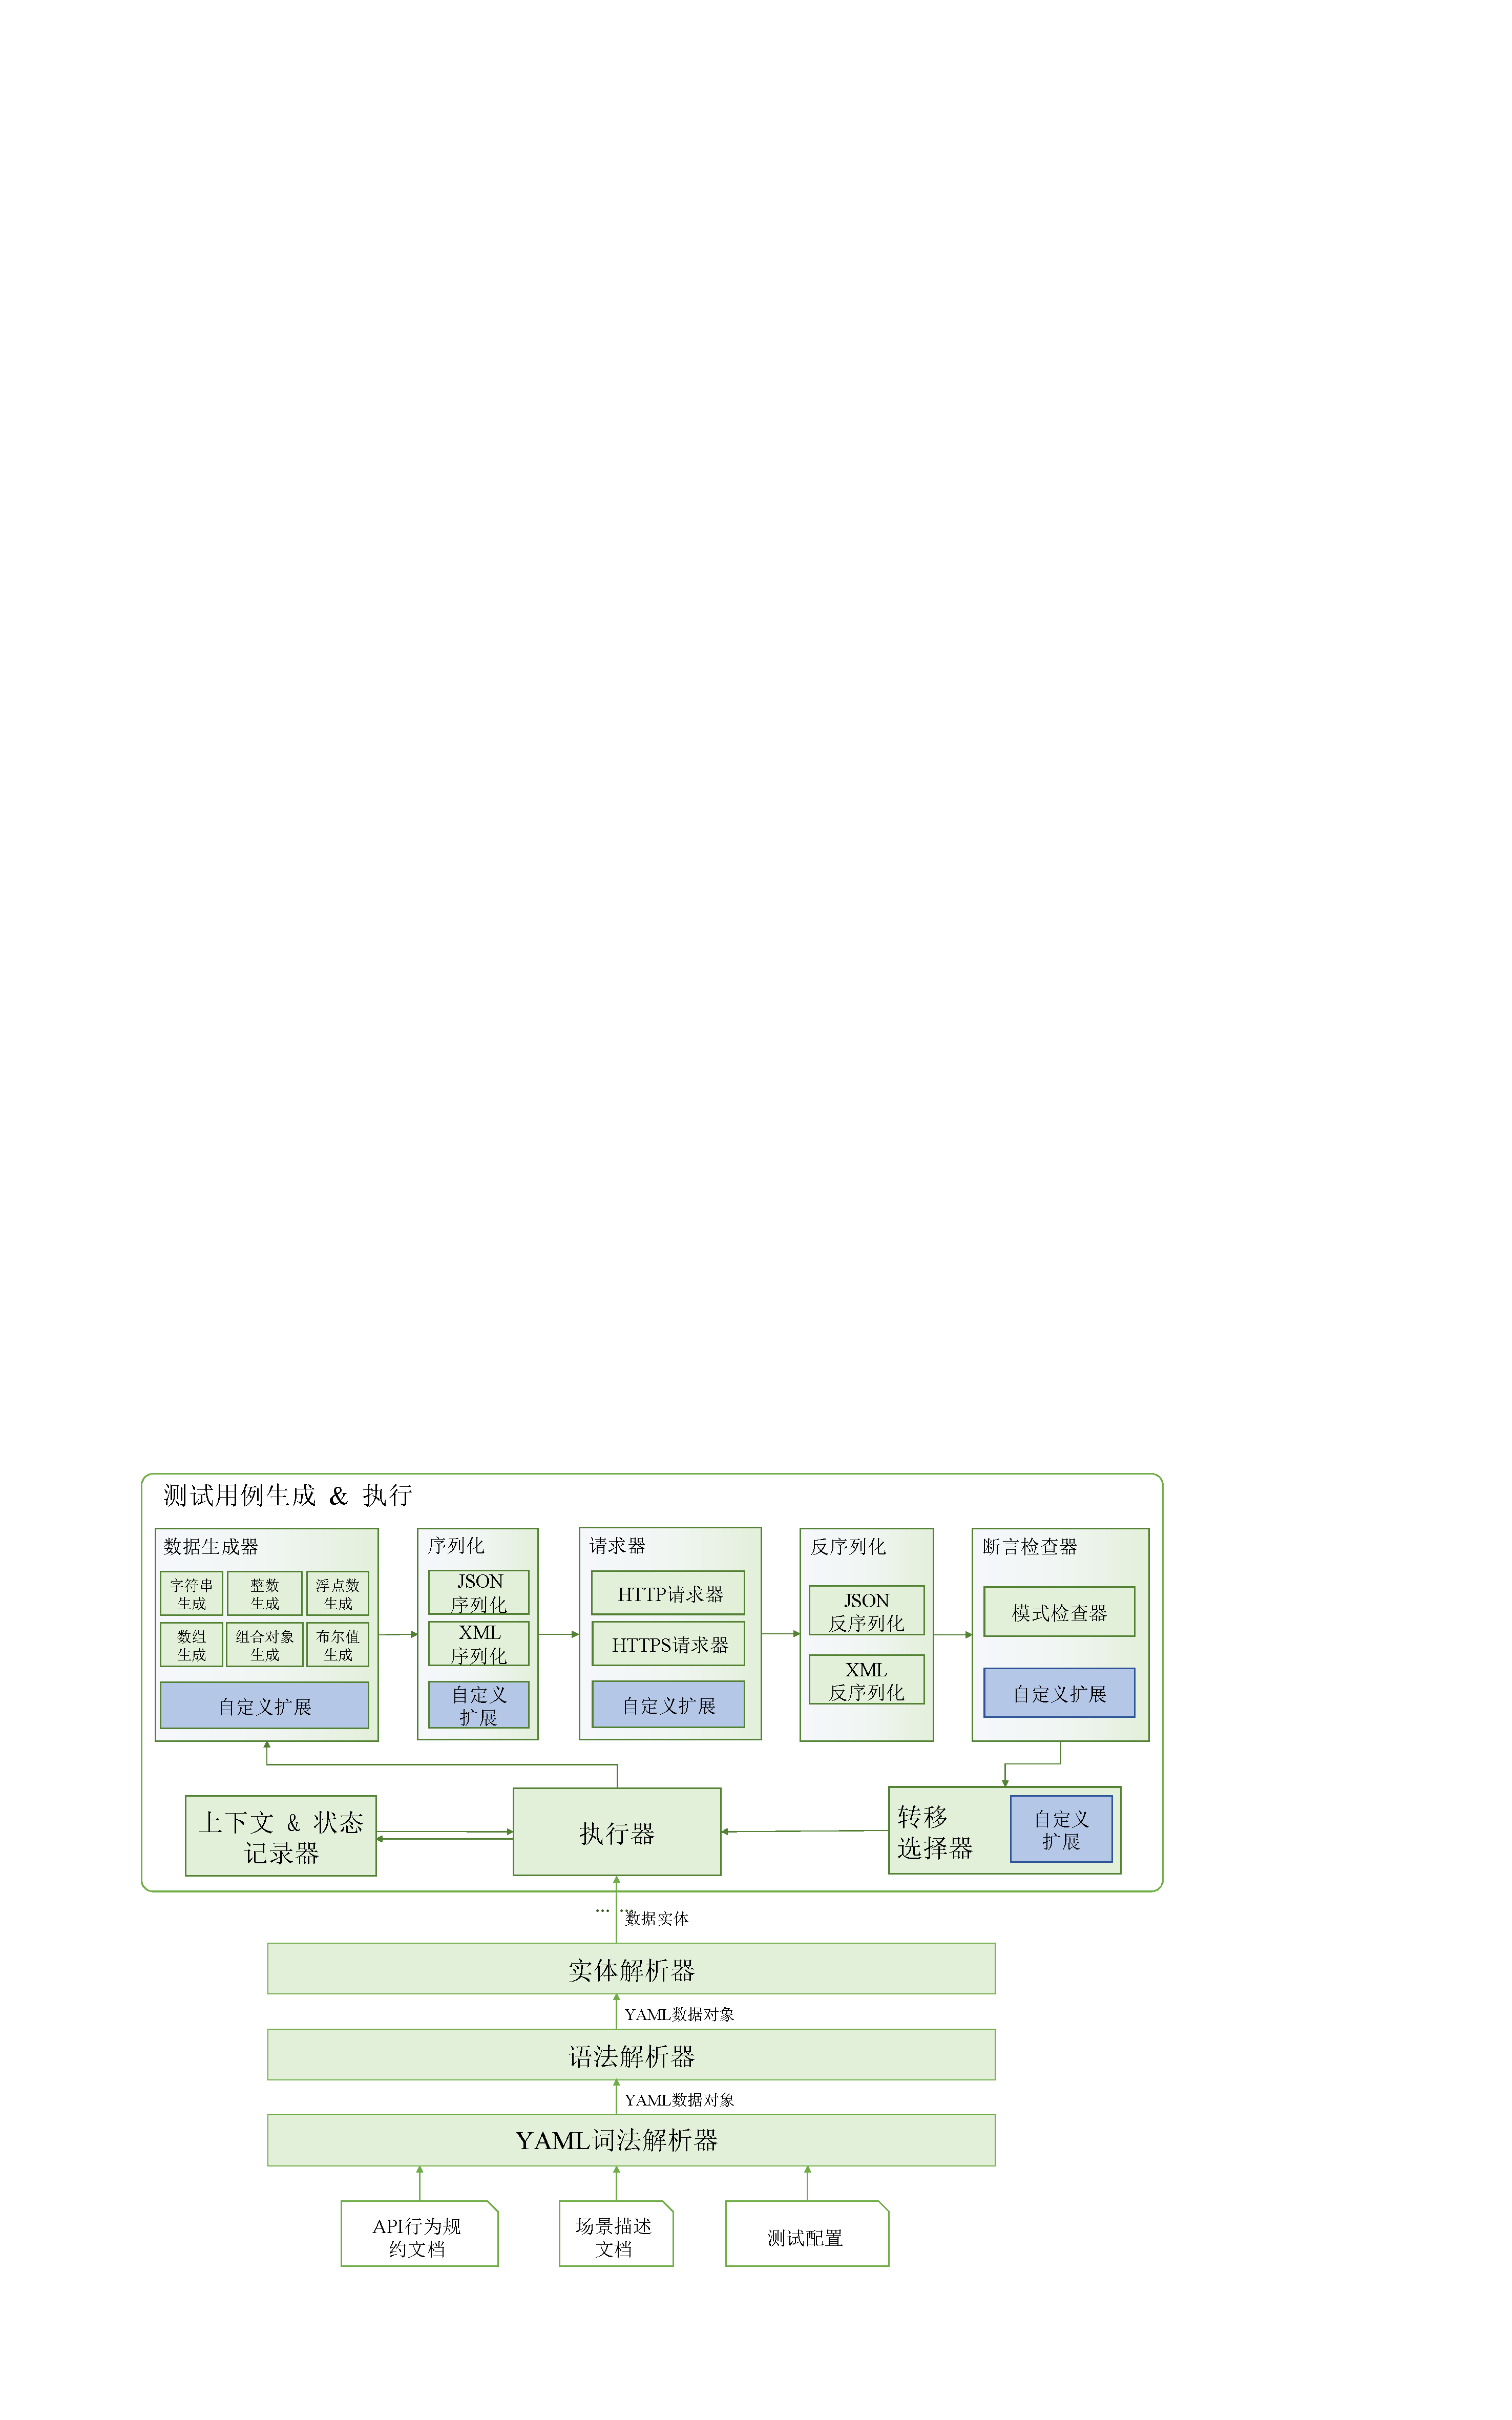
\includegraphics[width=400pt]{tool_architecture3.pdf}
	        \caption{Lapis工具整体架构. 工具的输入为OpenAPI语言描述的API行为规约文档, 场景描述文档和测试配置. 输出为测试用例及其执行结果. 数据流与执行流在图中从下往上, 从左往右.}
	        \label{fig:lapis_arch}
	    \end{figure}
	    
	    \label{sec:lapis_impl}
	    
	    图\ref{fig:lapis_arch}展示了Lapis工具的整体架构.
	    
	    工具提供C++与Python 3两个版本的实现. 其中C++版本效率较高, 但不支持用户扩展与自定义函数的引入. 本文主要以Python 3实现的版本进行工具介绍, 该实现其依赖于一些Python开源库, 如Requests\footnote{http://docs.python-requests.org}, PyYAML\footnote{https://pyyaml.org}, rstr\footnote{https://pypi.org/project/rstr/2.1.1}, 以及标准库.
	    
	    工具采用模块化的设计, 具有良好的可扩展性, 如图\ref{fig:lapis_arch}所示, 多个模块均支持用户自定义, 自定义函数和子类的引入得益于Python作为一门动态语言的反射机制, 要求这些自定义扩展使用Python实现.
	    
	    工具的输入为三个脚本文件 - 使用OpenAPI规约语言描述的API行为文档, YAML格式的场景模型文档, 以及YAML格式的测试配置文档. 本工作定义了一套格式规范, 用于表述场景模型. 测试配置文档为可选项, 内容较简单, 对API行为文档进行了一定补充, 并提供定制运行参数的功能. 三个脚本文件具有一定的层次关系: API行为文档提供了API的具体描述, 包括请求数据, 响应数据, 请求方法, 请求URL, 请求协议等; 场景模型文档利用这些信息, 并将场景模型的状态与对应API描述关联起来, 同时为自动化测试提供具体的场景模型; 测试配置文档则提供少量运行所需参数, 并支持一些可定制选项, 如指定测试用例生成与执行的时间限制等.
	    
	    工具的输出为包含所有测试用例及其执行结果的Python列表, 列表的各个元素即为各个测试用例, 包括测试用例的执行序列, 生成的请求数据, 获得的响应结果, 响应时间及模型覆盖率等信息.
	    
	    \label{sec:program_interface}
	    用户可以通过调用编程接口直接使用Lapis工具. 编程接口为Python函数的形式, 封装并隐藏了工具实现的具体细节. 普通用户使用\texttt{run()}函数, 即可一行完成测试生成与执行. \texttt{run()}函数的签名如下:
        \begin{flushleft}
            \scriptsize
            \tt
            \begin{lstlisting}[language=python]
def run(api_doc_path, scenario_doc_path, testconf_doc_path=None, num_case=1, verbose=0)
            \end{lstlisting}
        \end{flushleft}
        输入的三个脚本文件路径分别对应函数的前三个参数(测试配置脚本可选), 此外, 还可以指定生成测试用例的总数, 以及往控制台输出信息的详细级别. 函数的返回值即为工具的输出.
        
        下面对Lapis进行分模块介绍.

	    \subsection{词法解析器与语法解析器}
	        词法解析器分析输入的三个脚本文件的格式, 检查它们是否为合法的YAML文档, 并以数据对象的形式表示文档的层次结构, 数据对象使用\texttt{string}, \texttt{int}, \texttt{float}, \texttt{list}, \texttt{dict}等Python元素表示对象. 此模块基于PyYAML库实现, 对于不合法的YAML文档, 会通过错误提示机制告知不合法处的行号与列号.
	        
	        语法解析器则着重检查语义合法性, 如每个数据对象的必需域是否包含完全, 各个域的数据类型和取值是否合法等等. 此外, 脚本中允许使用\texttt{\$ref}域指明路径进行交叉引用, 语法解析器会进行解引用操作方便后续处理.
	    
	    \subsection{实体解析器}
	        实体解析器使用经过语法解析的数据对象作为输入, 提取对自动化测试有用的描述信息. API行为描述脚本中, 与请求发送相关的信息, 以及请求数据和响应数据的模式定义信息均被提取出来. 而如开发者联系方式域(\texttt{info.contact}域)等无关域则被舍去. 场景模型脚本和测试配置脚本的全部信息均被提取与转储.
	        
	        此外, 实体解析器还会进行一系列高级跨脚本的语义检查. 如, 在场景脚本中, 一个状态关联的API服务端点可以使用\texttt{OperationRef}和\texttt{OperationId}两个域指定, 实体解析器首先检查这两个域是否同时存在, 同时存在会带来歧义, 是不合法的. 然后, 如果使用\texttt{OperationRef}指定, 则检查文档路径指向的是否是API描述文档中一个合法的API定义, 如果使用\texttt{OperationId}指定, 则检查其是否在之前遍历API描述脚本时记录的API ID列表里. 最后, 如果检查通过, 则将关联的API服务端点的信息实例赋给此状态实例.
	        
	        提取与转储的描述信息, 经过实体解析器处理, 就不再使用数据对象存储了, 而是使用对应的Python类实例存储. 如\texttt{Operation}类, \texttt{Scenario}类, \texttt{Response}类等等. 各个信息域是类的成员变量. 这种方式为数据的传递施加了类型限制, 更加清晰.
	    
	    \subsection{测试执行}
	    
	        测试执行模块是工具的核心模块, 其各个子模块的功能如下:
	        
	        \begin{itemize}
	            \item 测试执行器:\\
    	            测试执行器调度和控制整个测试用例的生成和执行过程. 它实现了基于场景模型的执行序列生成算法(算法\ref{algo:seqgen}). 执行器也负责处理用户自定义扩展抛出的异常, 防止系统崩溃. 用户调用的编程接口直接与此模块进行交互.
    	            
	            \item 上下文\&状态记录器:\\
	                此模块记录测试的所有有价值信息, 最后返回给用户.
	                
	            \item 数据生成器:\\
	                此模块根据合法请求数据定义和请求数据依赖定义生成请求参数, 实现了\ref{sec:req_data_gen}所述的请求数据生成方法. 在该子模块中, 可以通过用户扩展引入自定义生成函数.
	                
	            \item 序列化:\\
	                此模块将生成的请求参数序列化/格式化为字符串. 除了默认的JSON格式和XML格式序列化模块外, 用户也可以用子类化的方法, 实现自定义的序列化格式;
	                
	            \item 请求器:\\
	                此模块发送请求, 并收集响应结果. 负责处理网络交互的细节. 为了支持各种不同的API服务, 除了已实现的HTTP协议缺省请求器和HTTPS协议缺省请求器外, 用户还可以通过子类化抽象接口类的方法编写自定义请求器. 如, 通过这种方式, 对使用签名机制的API使用专用请求器.
	                
	            \item 反序列化:\\
	                此模块将响应的头和响应体分离, 并根据API行为文档和测试配置文档中的数据格式定义, 将字符串解析为数据实体.
	                
	            \item 断言检查器:\\
	                此模块对响应数据进行检查, 它包括模式检查(是否符合合法响应数据定义)和断言检查(检查是否满足响应断言定义)两个方面. 在该子模块中, 可以通过用户扩展引入自定义校验函数.
	                
	            \item 转移选择器:\\
	                此模块首先根据响应数据和各个转移上的条件确定可选转移集, 然后根据定义的概率决定是否终止执行或者选择出要执行的转移. 在该子模块中, 可以通过用户扩展引入自定义校验函数. 还可以通过实现接口函数并在测试配置文档中引入的方式, 在转移选择器中应用启发式转移选择算法.
	        \end{itemize}
	    
	        除了以上子模块外, 在全局测试配置中, 为了更好地与被测系统(SUT)交互, 测试执行模块提供了用于被测系统启动, 停止和请求间隔操作的函数接口, 在测试配置文档中指定函数的所在位置, 即可引入这些自定义交互函数.

	\section{脚本编辑工具}

        本文的工具与方法使用结构化的脚本文档作为输入, 脚本文档则常常需要手工编写, 因此, 用户友好的脚本编辑和管理工具不可或缺.
        
        \begin{figure}[!htb]
            \centering
            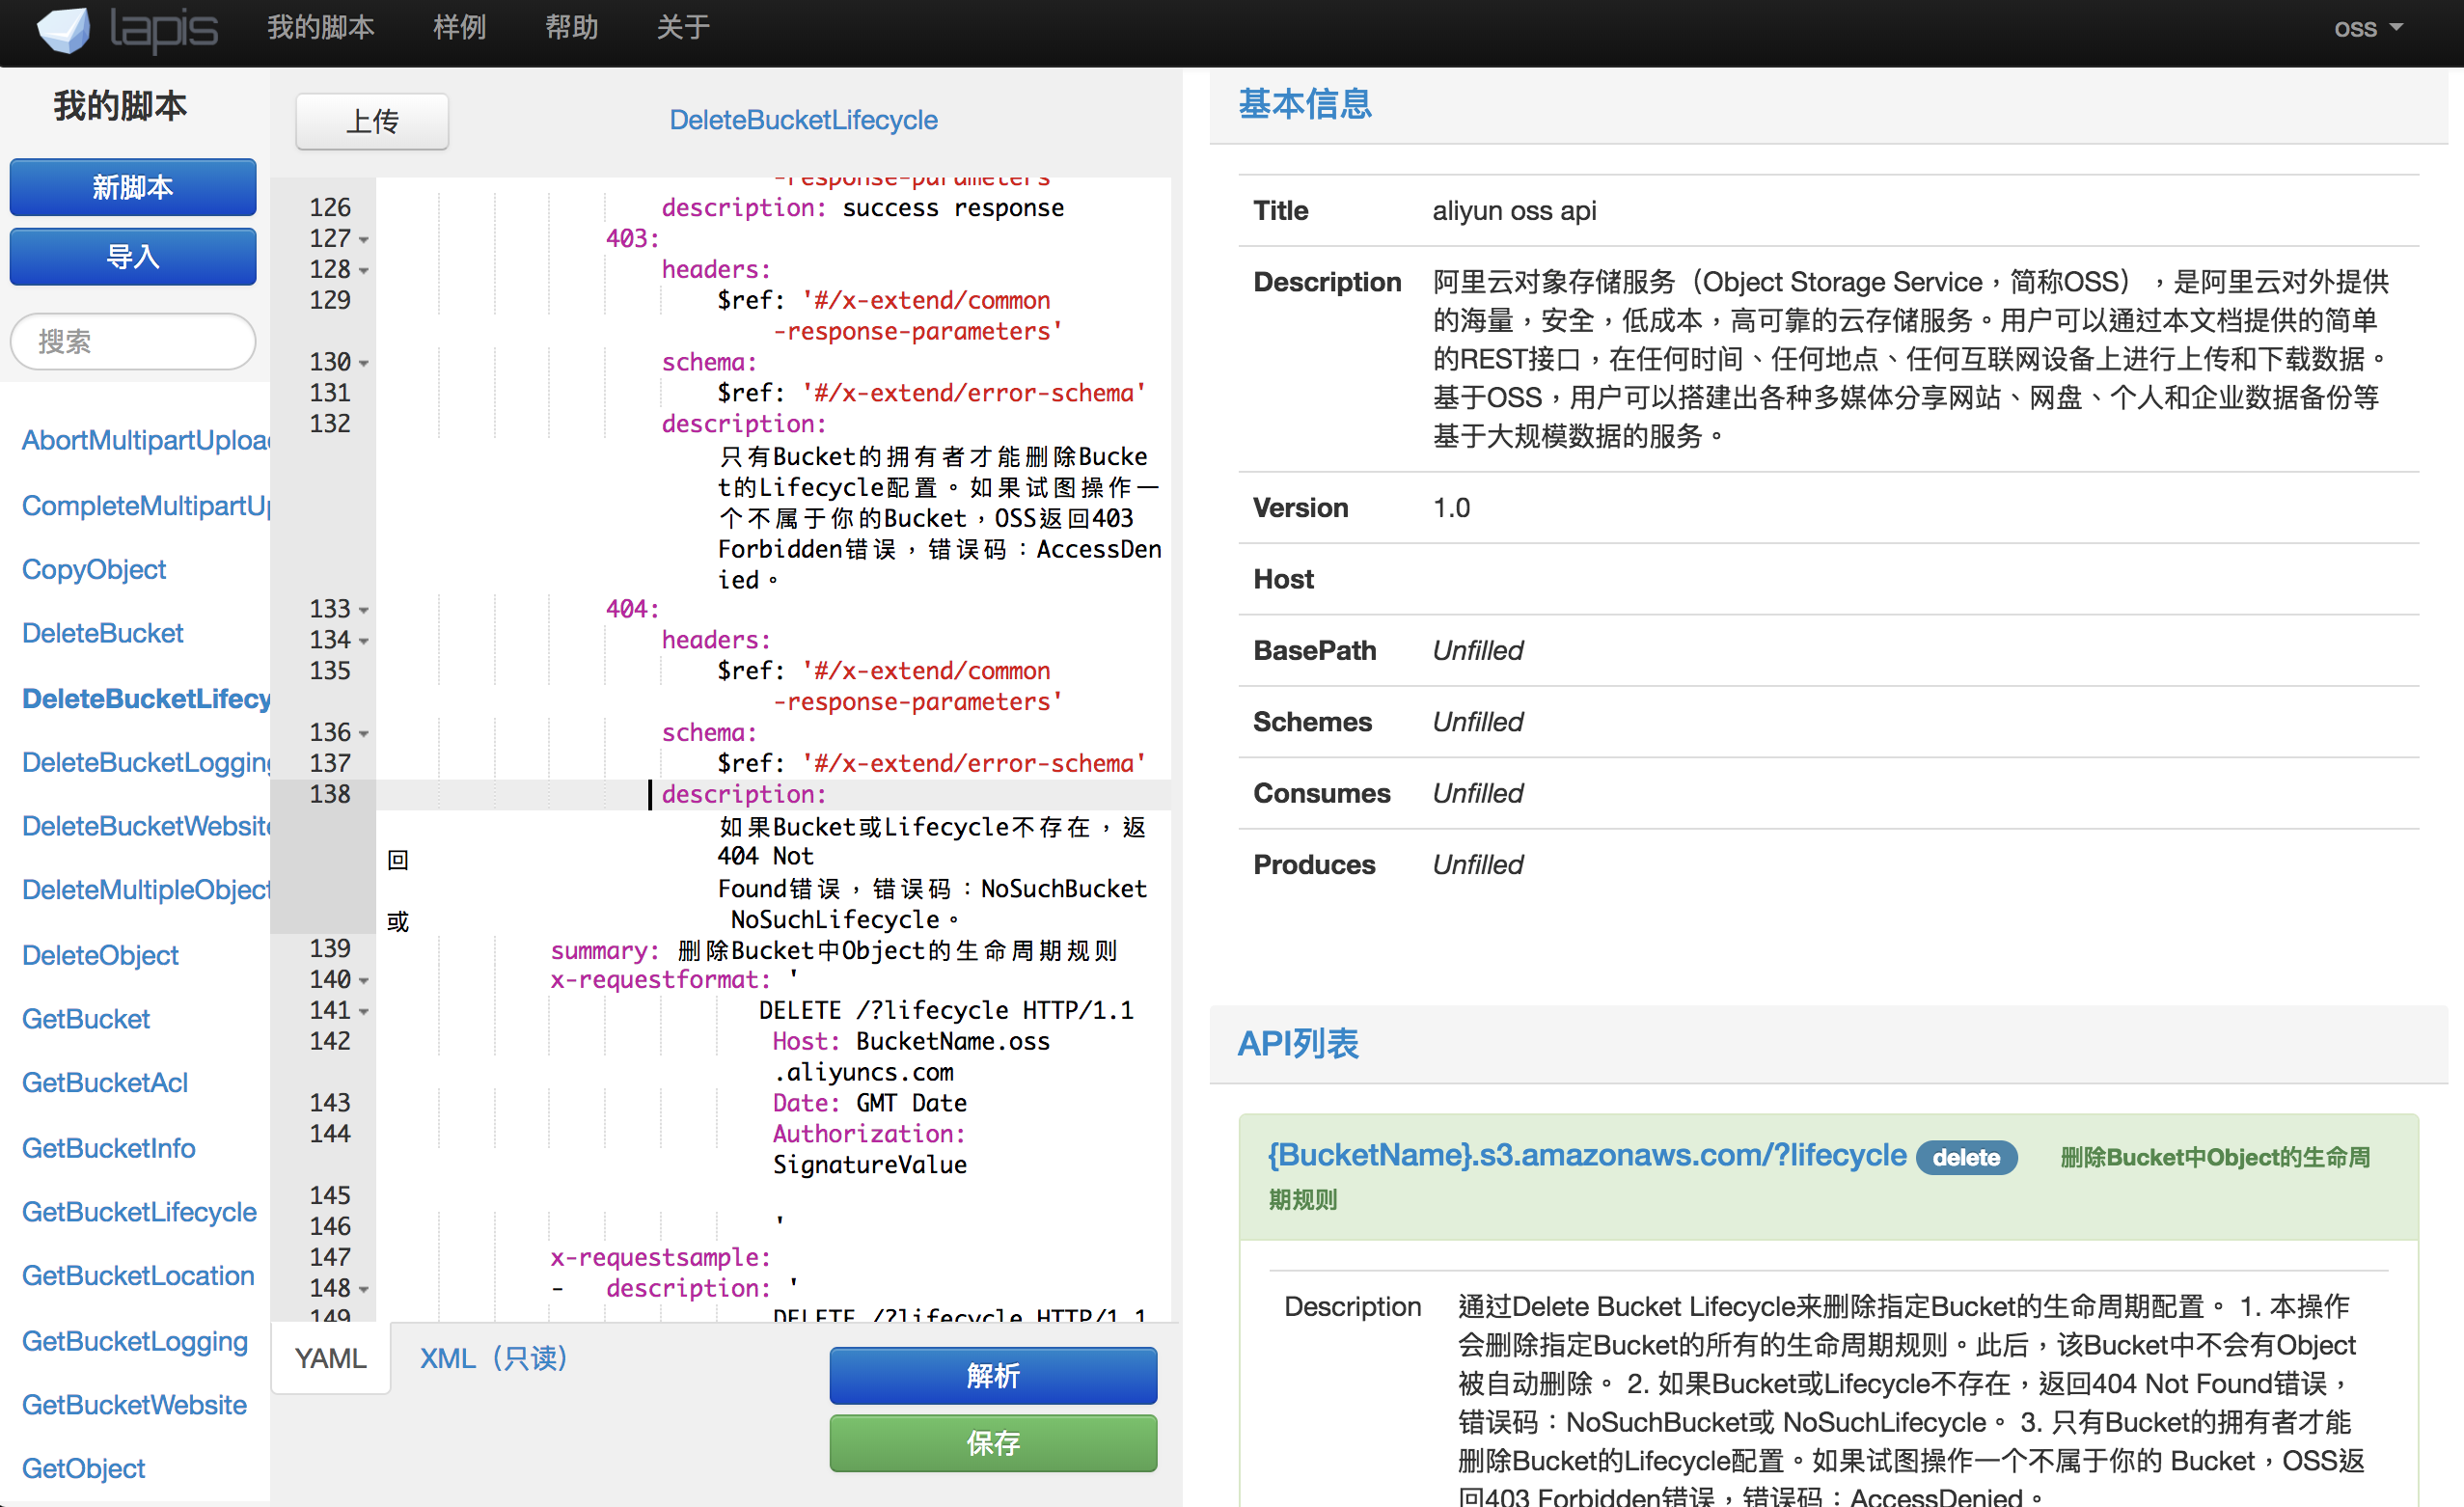
\includegraphics[width=300pt]{frontend_screenshot.png}
            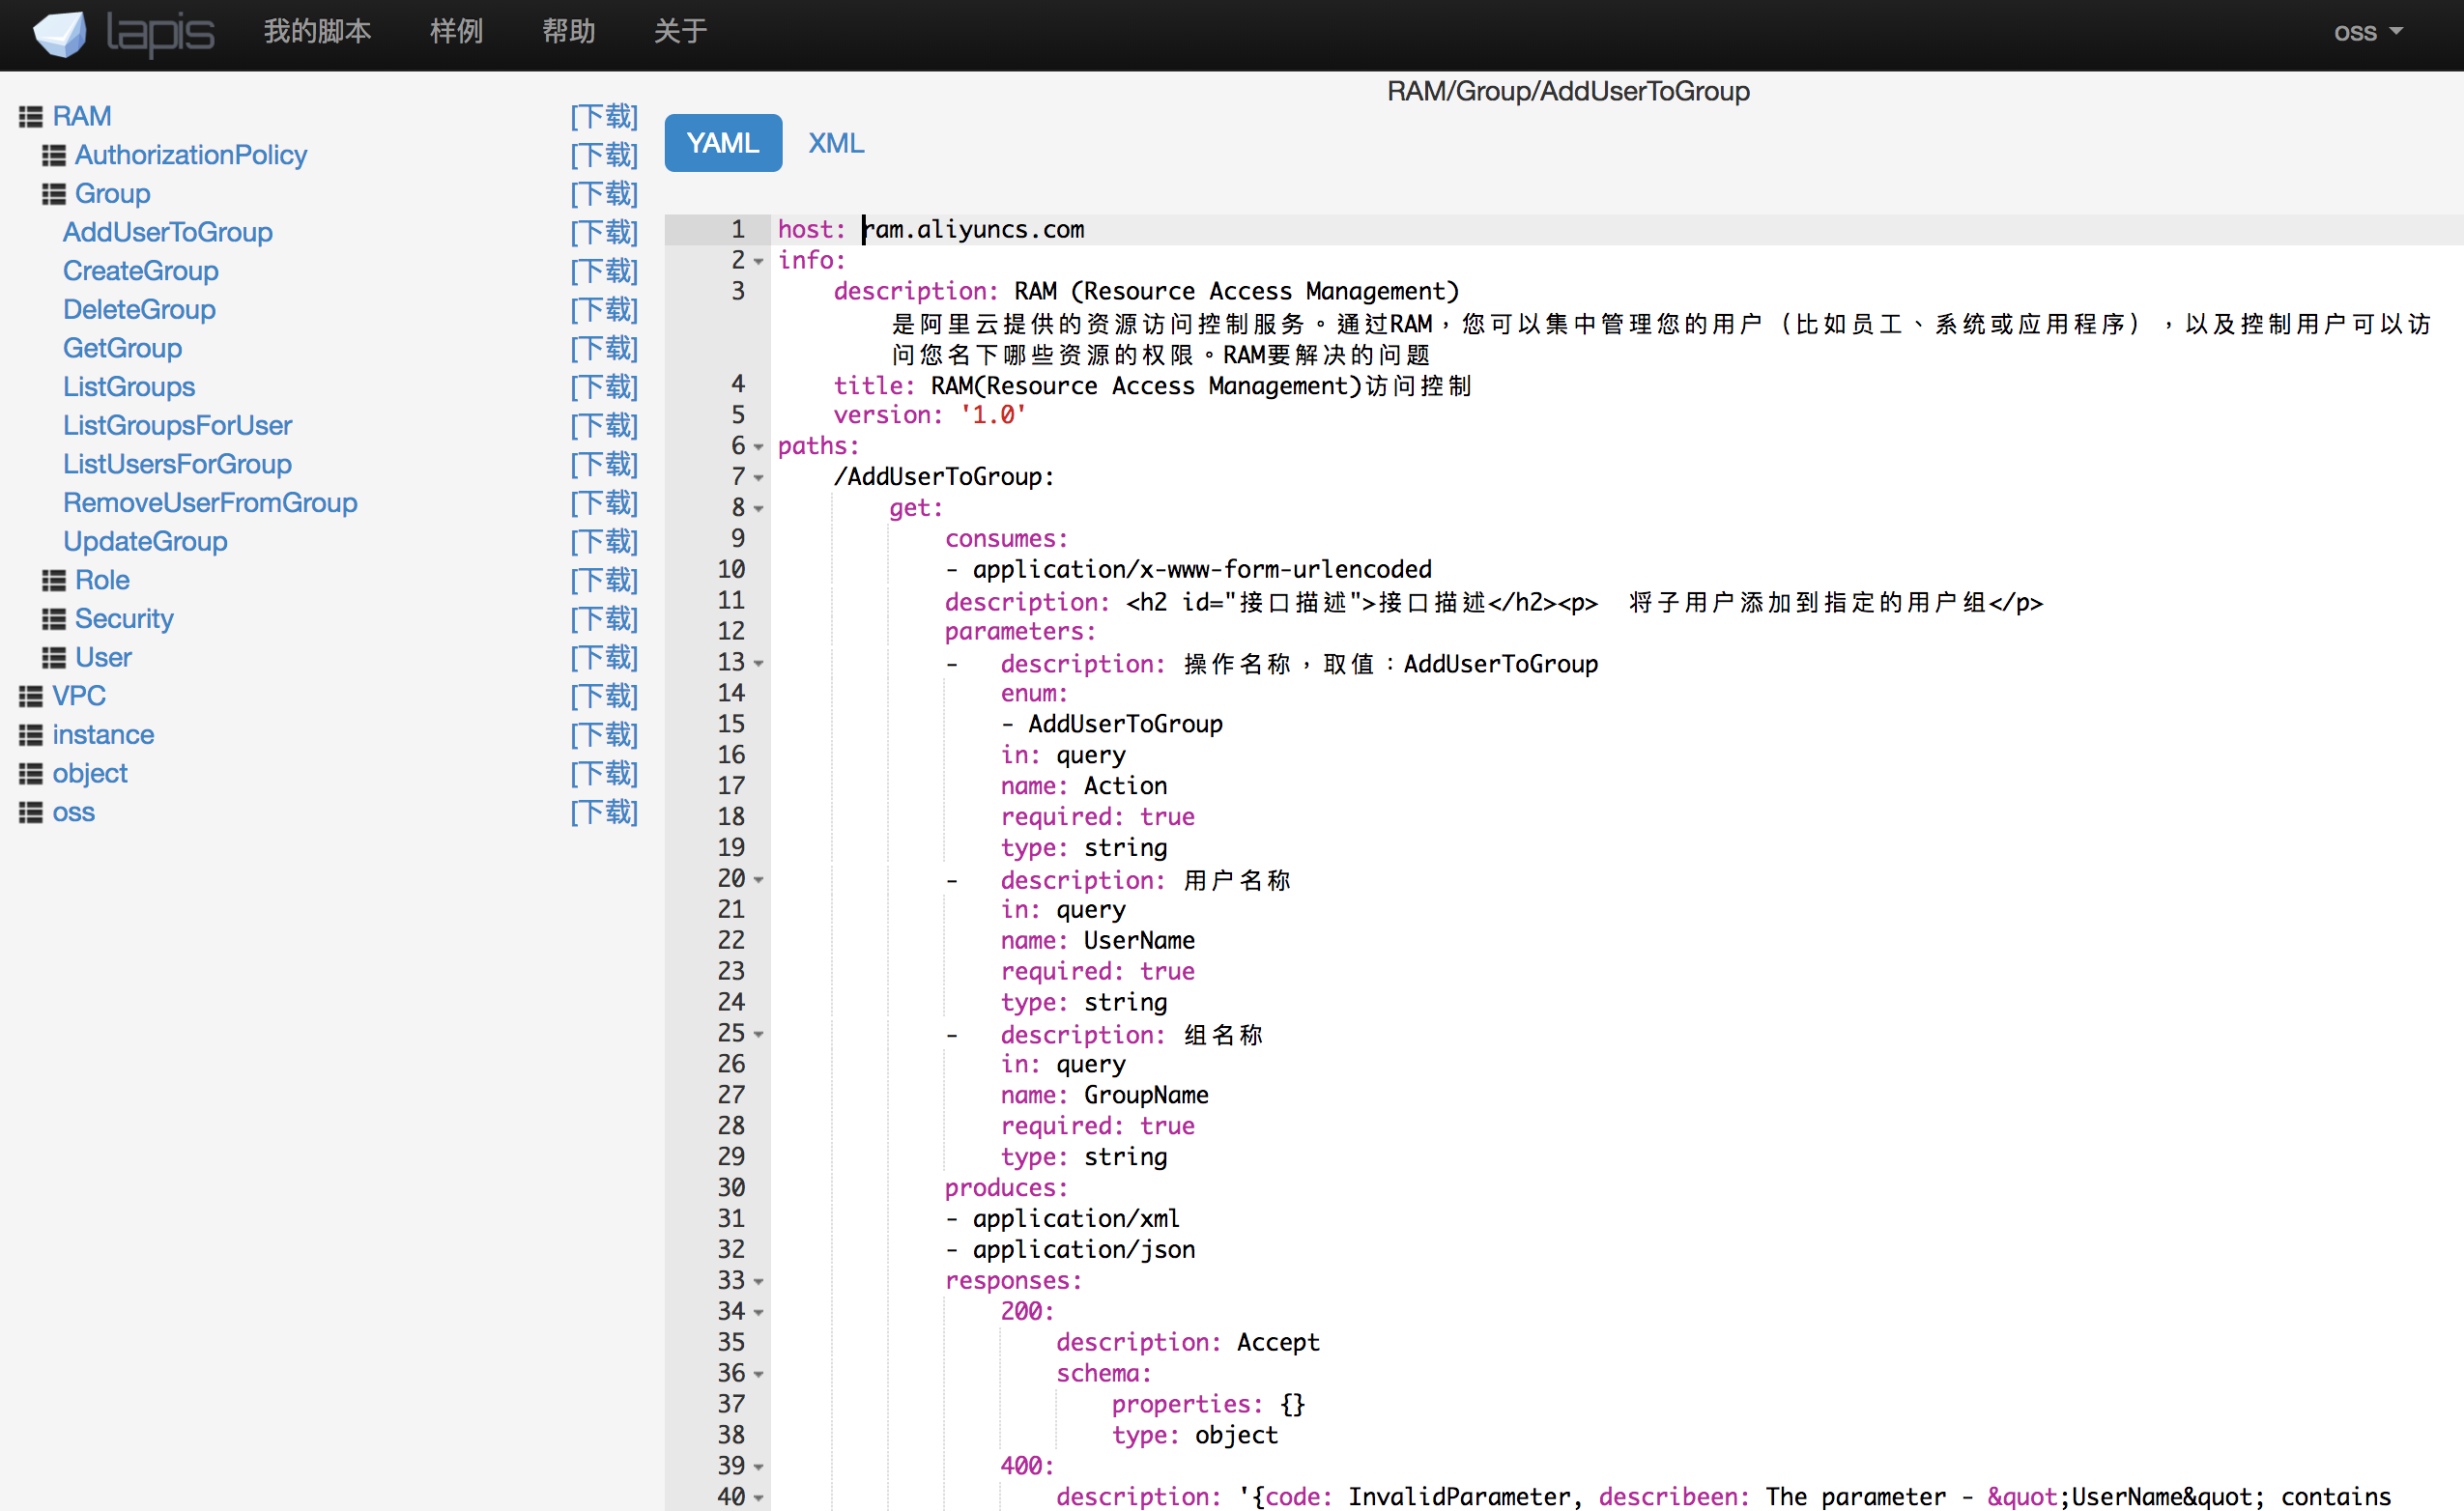
\includegraphics[width=300pt]{frontend_screenshot2.png}
            \caption{Web端脚本编辑工具前端截图. 通过此工具, 用户可以在线进行脚本的编辑与上传. 编辑时, 工具对API脚本进行实时解析, 以类似于API使用手册的形式展示脚本内容.}
            \label{fig:frontend_screenshot}
        \end{figure}
        
        本工作为OpenAPI格式的API行为文档的编辑与管理开发了一个在线web工具, 运行截图见图\ref{fig:frontend_screenshot}. 在此工具中, 用户可在线编辑与上传API行为文档, 并获得解析结果的实时反馈. 如果文档的内容合法, 前端会将所描述的API以类似于使用手册的形式进行可视化, 并展示于右栏. 为了提升可读性, 各个参数和响应体的展示采用折叠式的设计. 如果文档的内容不合法, 工具会提示出错原因与位置. 每个注册用户拥有私有文件夹, 后台记录了文件夹内各文档的历史版本, 文档也可从本地上传到此文件夹. 此外, 编辑工具还附带大量样例方便用户快速熟悉文档采用的OpenAPI规约语言.
        
        此web编辑工具的后端采用Python语言和Django框架, 前端采用JQuery和Bootstrap库. 直接依托文件系统实现了用户和文档托管功能, 无数据库依赖, 较轻量, 适合部署作为企业测试部门内部服务或单机使用.
    
        \begin{figure}
            \centering
            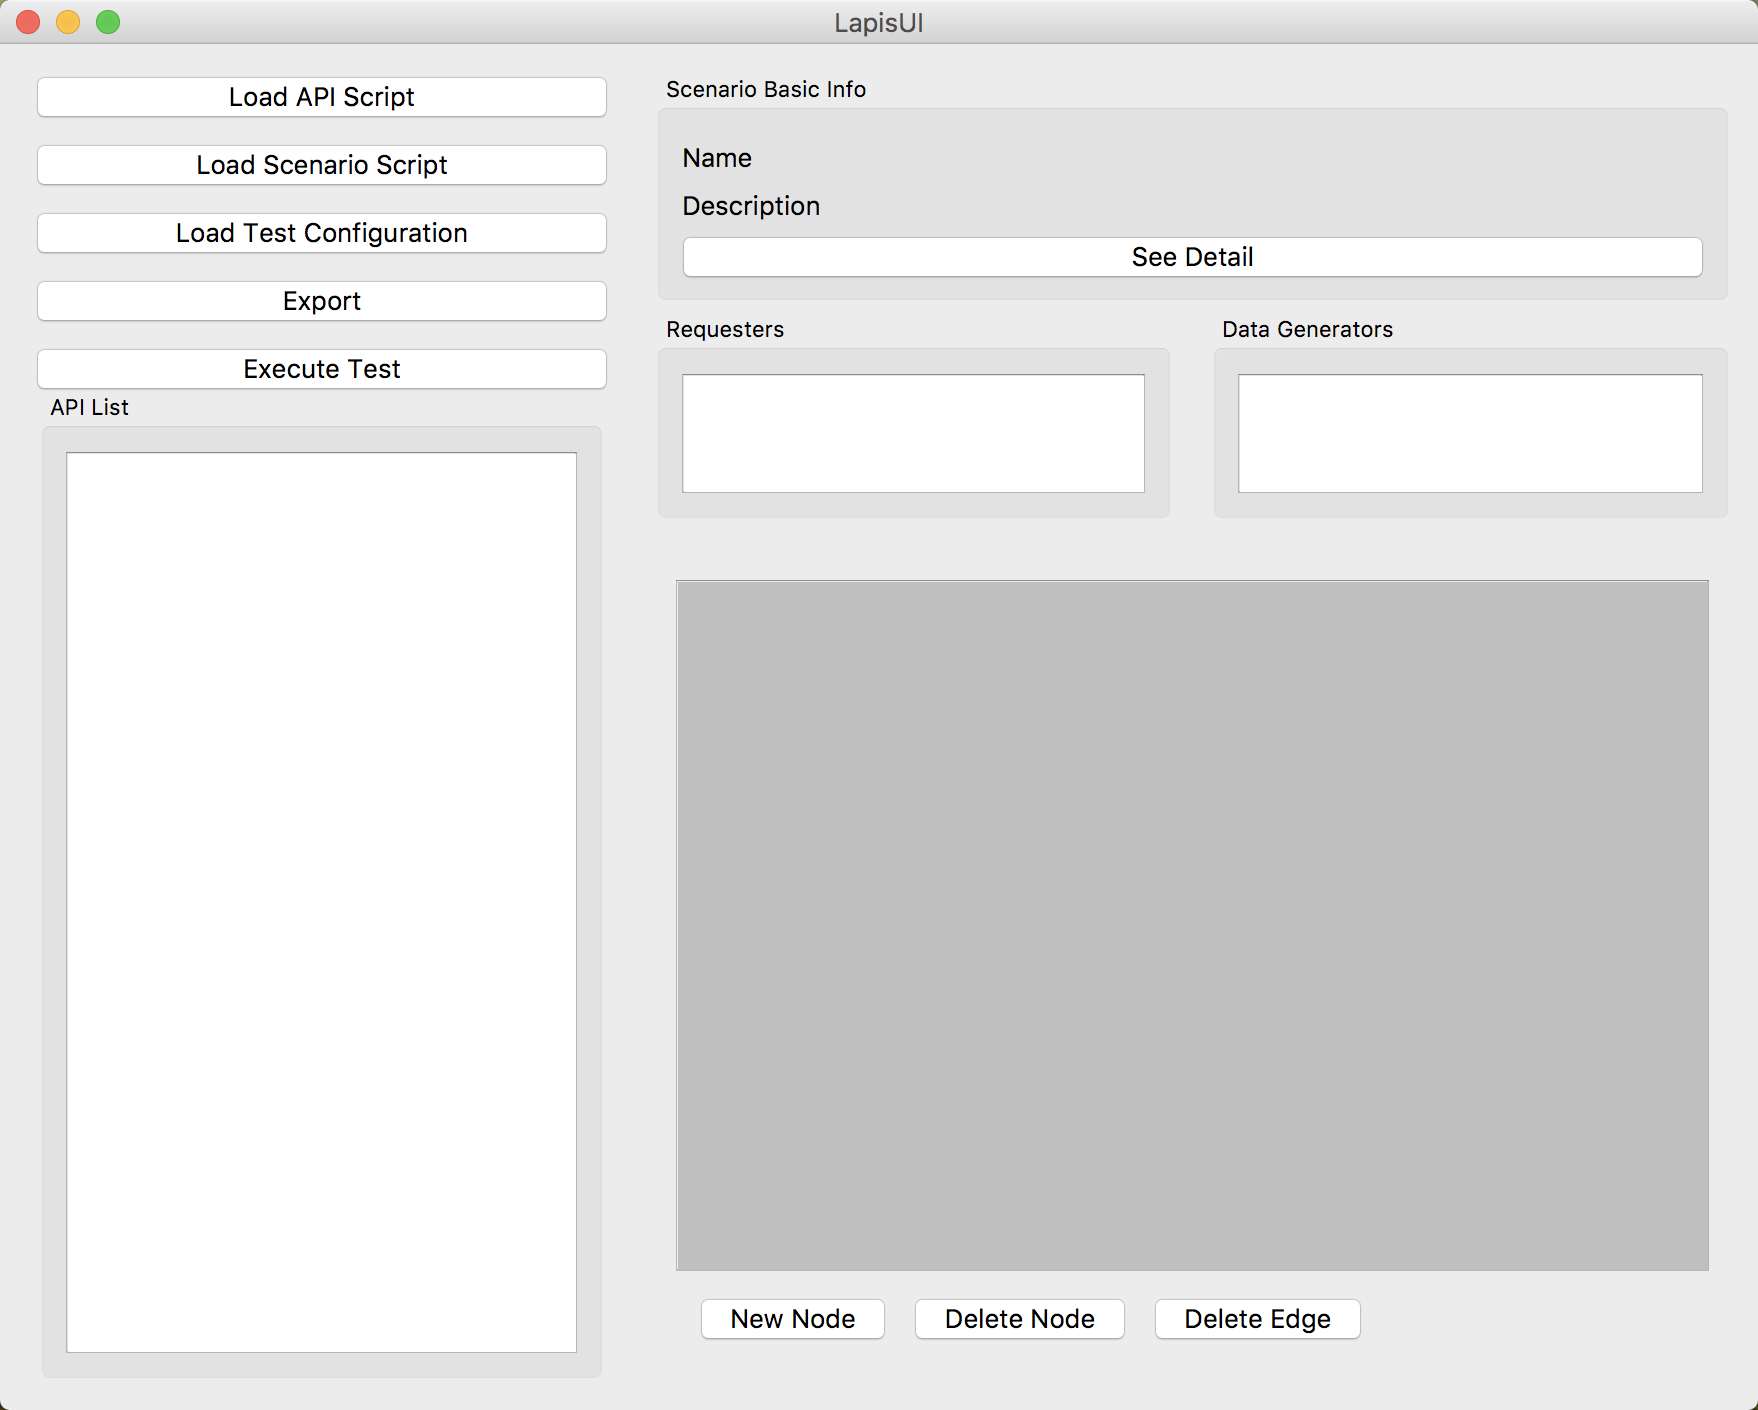
\includegraphics[width=300pt]{LapisUI.png}
            \caption{LapisUI系统截图.}
            \label{fig:lapis_ui_screenshot}
        \end{figure}
    
        \label{sec:scenario_gui_edit}
        此外, 本文亦正在实现桌面端的场景综合编辑与管理系统. 该系统整合了Lapis工具的内部API, 让用户通过GUI, 进行包括API描述文档加载与查看, 场景模型加载与展示, 基于有向图的场景模型绘制与编辑等等功能. 系统旨在极大减少场景模型设计与分析的人工成本. 系统的设计借鉴了\inlinecite{junyiw17}的相关工作, 拟于近期完成. 目前工具的截图见图\ref{fig:lapis_ui_screenshot}.
        
    % extended version
	% \section{*桌面端测试管理系统}


